\chapter{研究結果}

\section{感測器檢測狀況}
\begin{figure}[H]
	\centering
	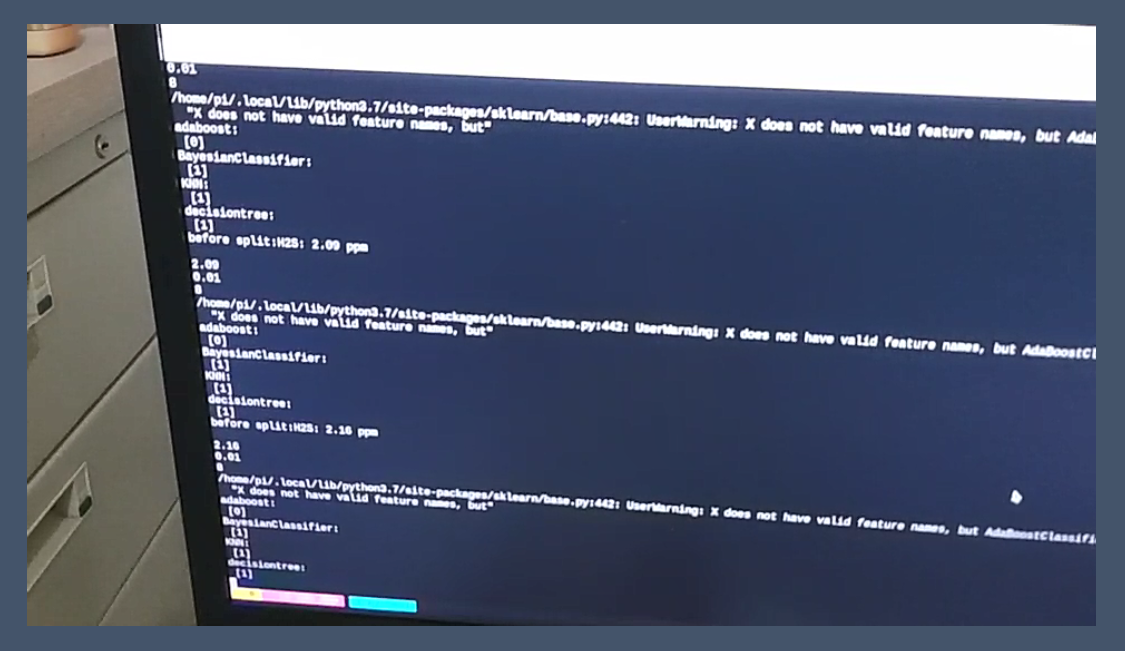
\includegraphics[width=0.8\textwidth]{pic/terminal_output.png}
\end{figure}
使用的三個感測器皆已成功完成線路連接,且能及時讀取氣體濃度,並且經由多種機器模型判斷後,輸出分類結果到螢幕(terminal)。

\section{模型時間準確度}
\begin{itemize}
	\item 決策樹
	\begin{figure}[H]
		\centering
		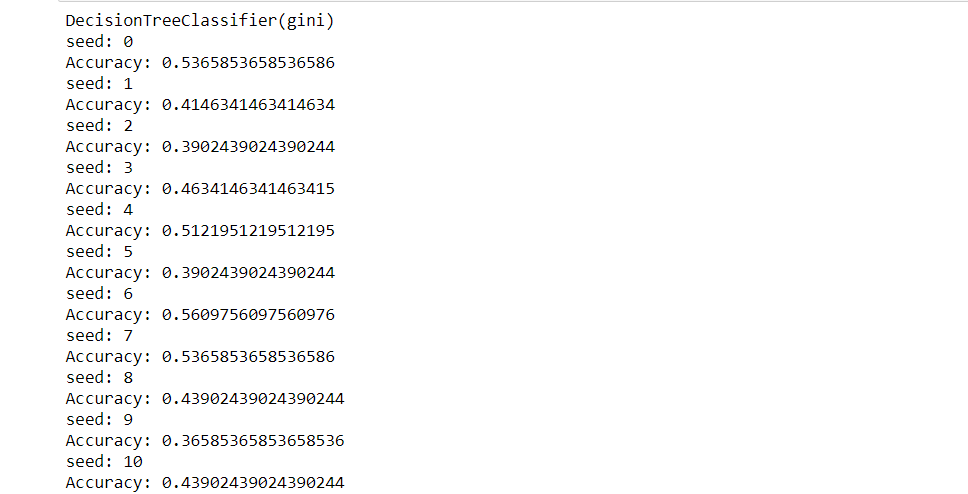
\includegraphics[width=0.8\textwidth]{pic/decisiontree.png}
	\end{figure}
	\item KNN
	\begin{figure}[H]
		\centering
		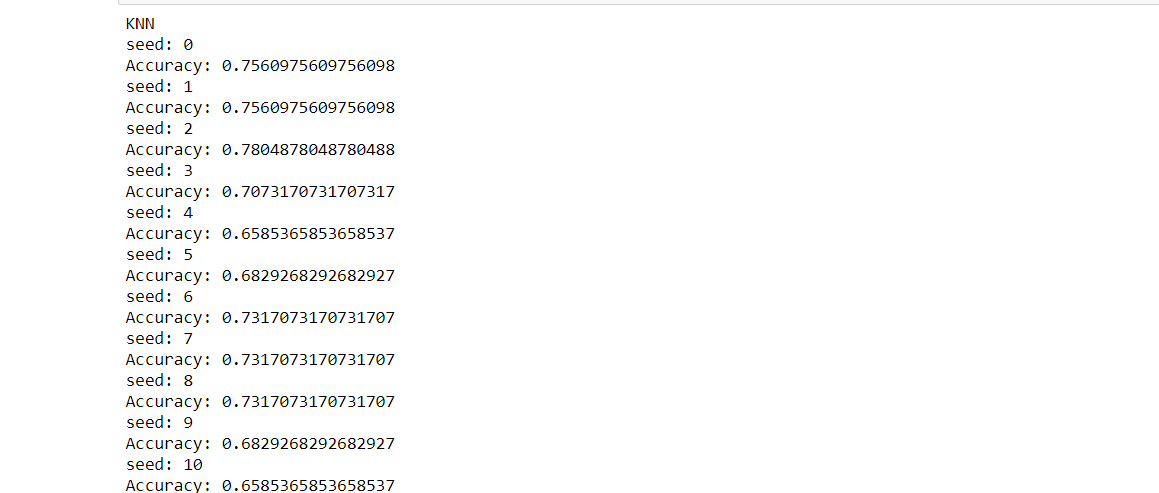
\includegraphics[width=0.8\textwidth]{pic/knn.png}
	\end{figure}
	\item 單純貝氏
	\begin{figure}[H]
		\centering
		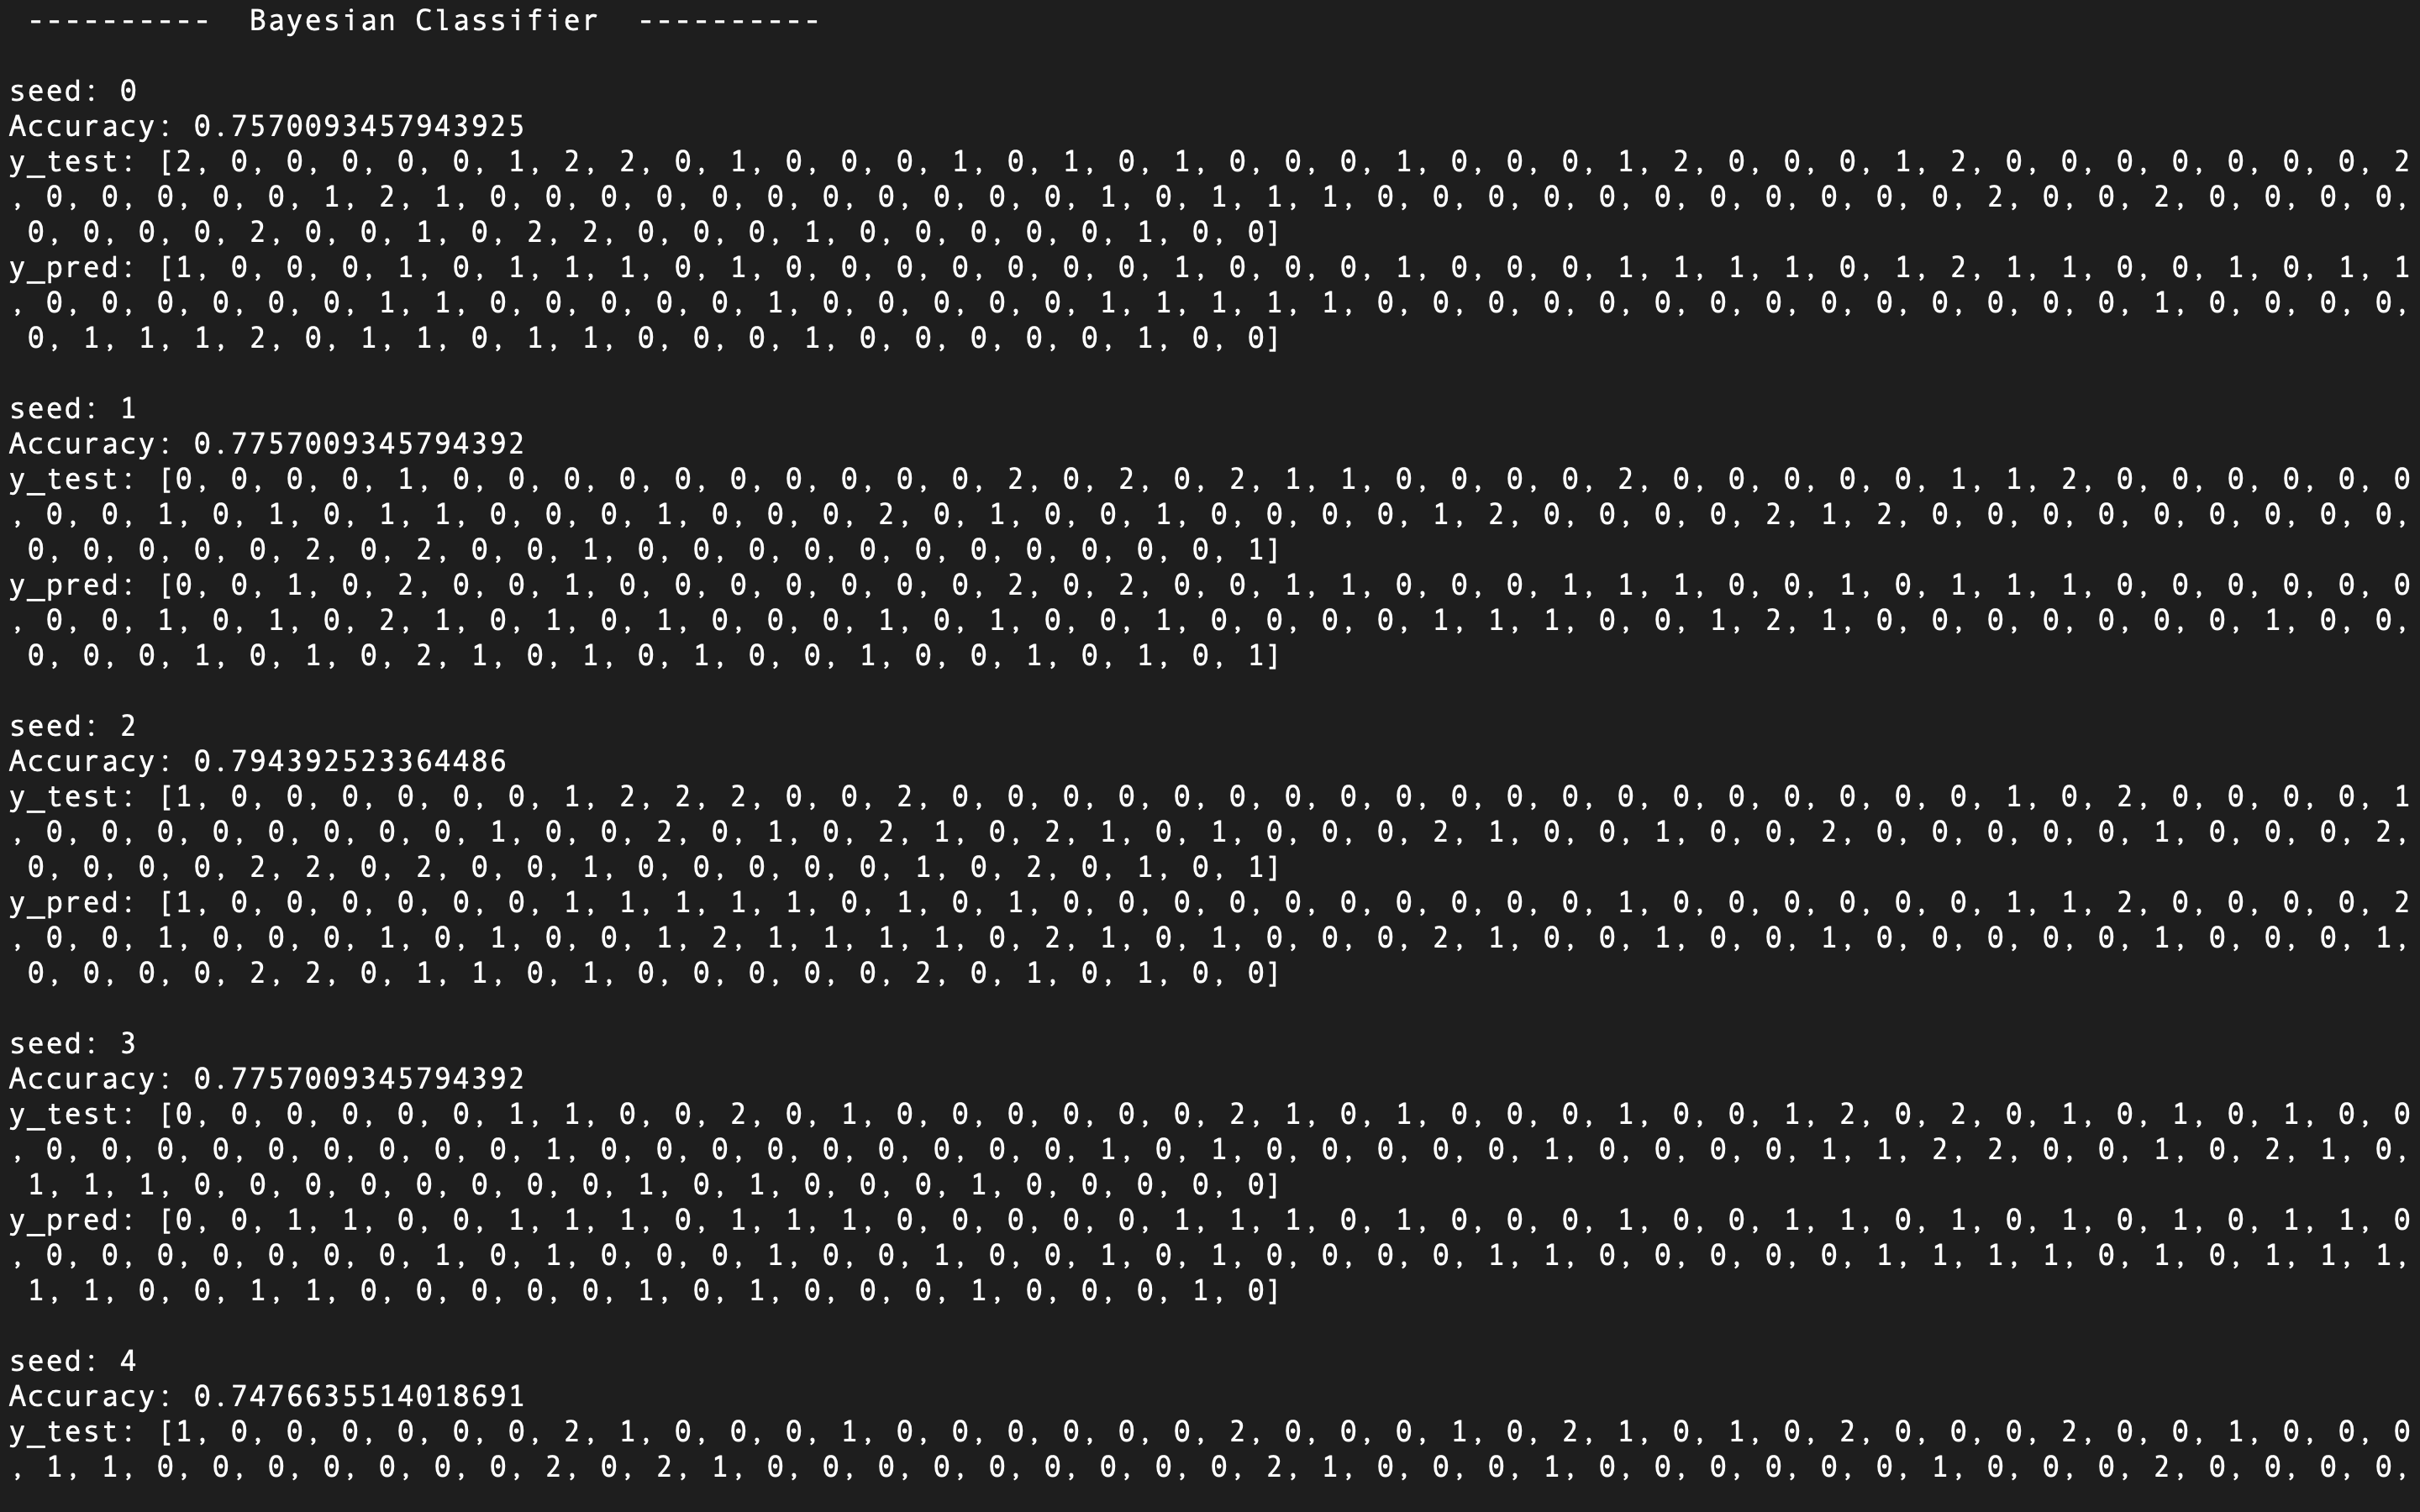
\includegraphics[width=0.8\textwidth]{pic/Bayesian.png}
	\end{figure}
	\item AdaBoost
	\begin{figure}[H]
		\centering
		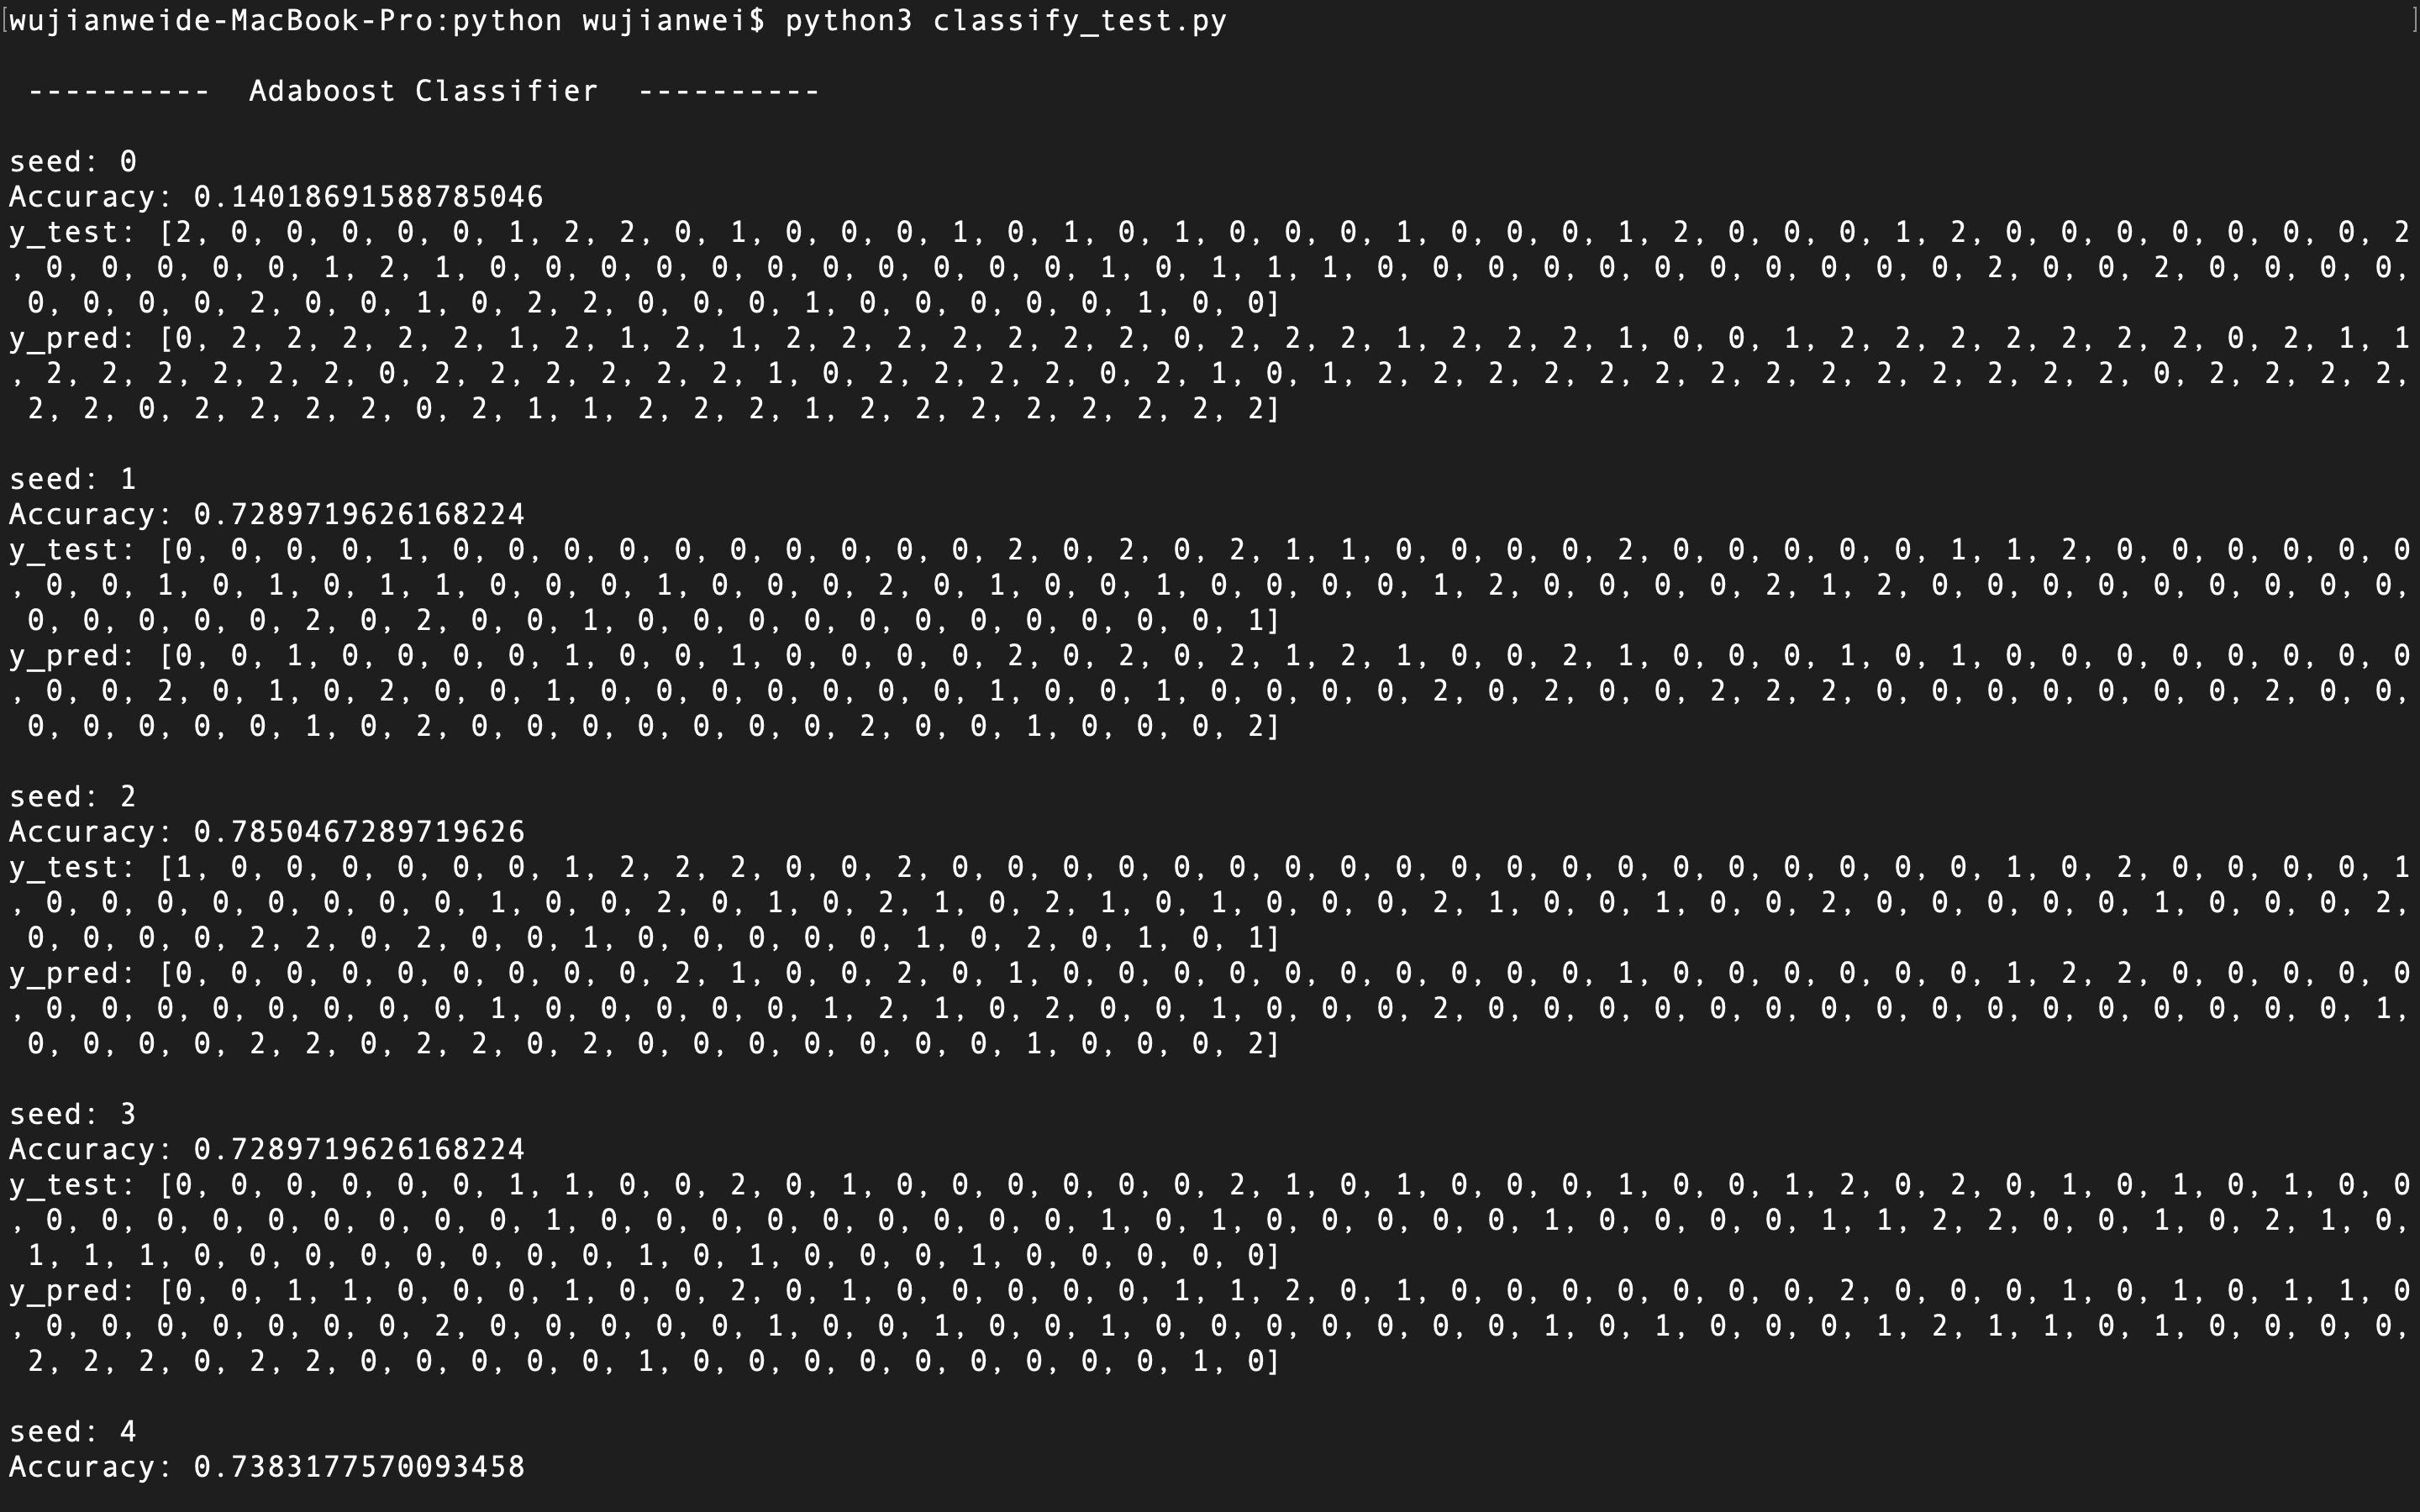
\includegraphics[width=0.8\textwidth]{pic/Adaboost.png}
	\end{figure}
\end{itemize}

\section{設備外型}
	\subsection{內層殼層}
		利用保麗龍盒,可以良好的隔絕外界溫度與氣體,使得實驗不會被外界空氣影響。
		\begin{figure}[H]
			\centering
			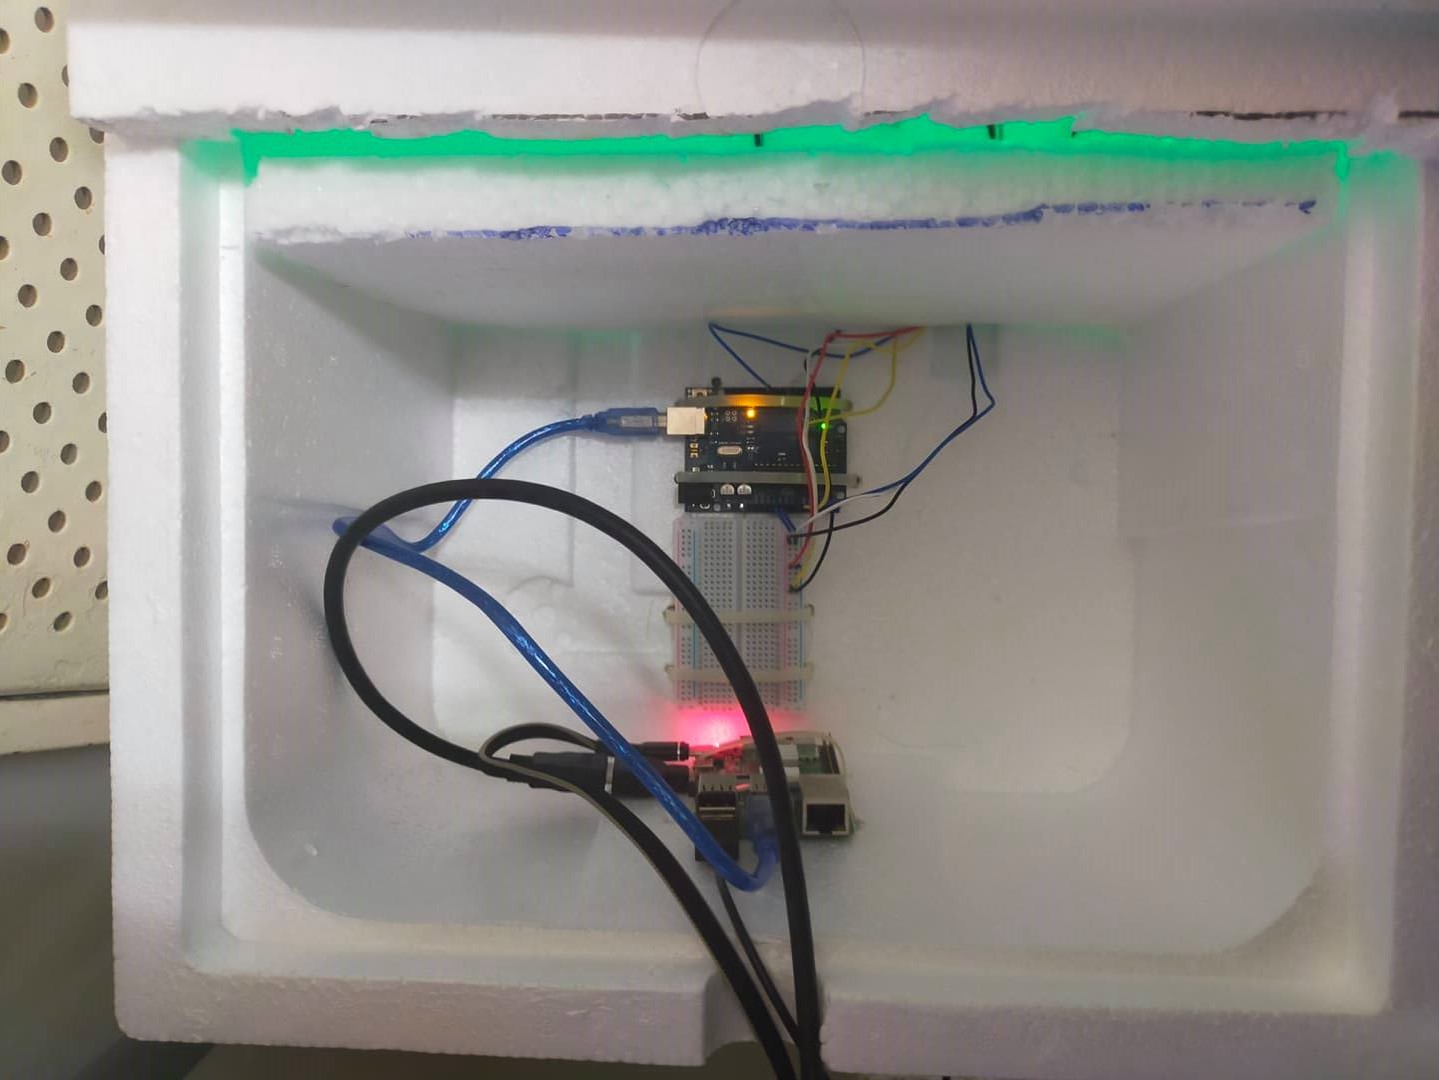
\includegraphics[width=0.5\textwidth]{pic/box(1).jpg}
		\end{figure}
		\begin{figure}[H]
			\centering
			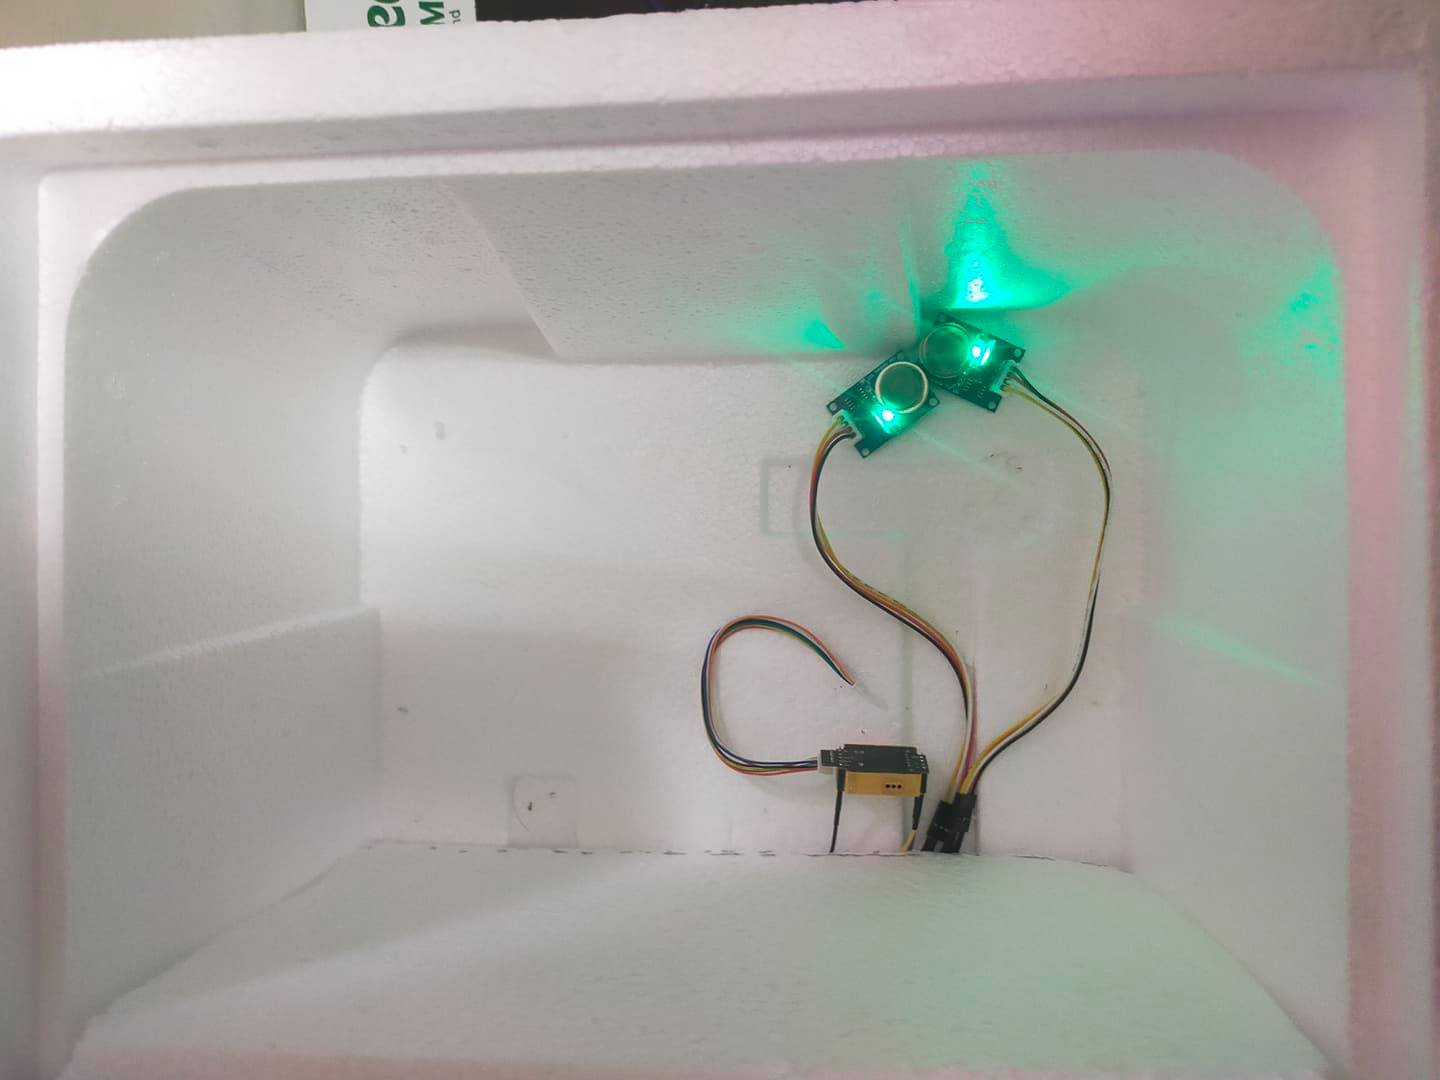
\includegraphics[width=0.5\textwidth]{pic/box(2).jpg}
		\end{figure}
		\begin{figure}[H]
			\centering
			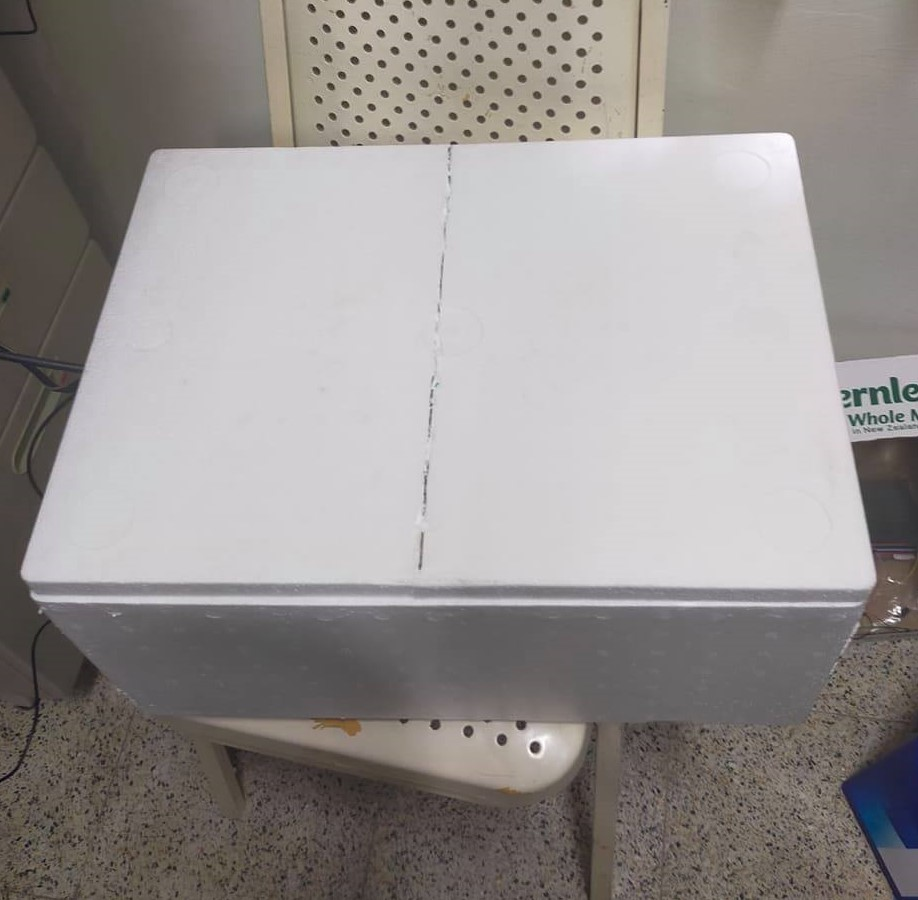
\includegraphics[width=0.5\textwidth]{pic/box(3).jpg}
		\end{figure}
	\subsection{外層水泥殼層加固}
		後來老師提示後,發現外殼強度不足,所以在外面加了一層水泥。水泥是成本較低,
		且能夠達到良好的保護作用,使得保麗龍盒子不容易受到損壞。
		\begin{figure}[H]
			\centering
			\includegraphics[width=0.5\textwidth]{pic/concrete_box1.jpg}
		\end{figure}
		\begin{figure}[H]
			\centering
			\includegraphics[width=0.5\textwidth]{pic/concrete_box2.jpg}
		\end{figure}
		\begin{figure}[H]
			\centering
			\includegraphics[width=0.5\textwidth]{pic/concrete_box3.jpg}
		\end{figure}

\section{氣體相關性}
	\subsection{$CO_2$}
		二氧化碳在本次專題實驗數據中,相關性不高,因此後續不討論。
	\subsection{$NH_3$ \& $H_2S$}
		我們把實驗數據分成三個區間,在圖中也會以三種顏色表示:藍色表示 0 \textasciitilde \ 2 小時,紅色表示 3 \textasciitilde \ 6 小時,綠色表示 7 小時以上。
		從圖中可以稍微觀察到 $NH_3$ 和 $H_2S$ 之間略微有相關。
		\begin{figure}[H]
			\centering
			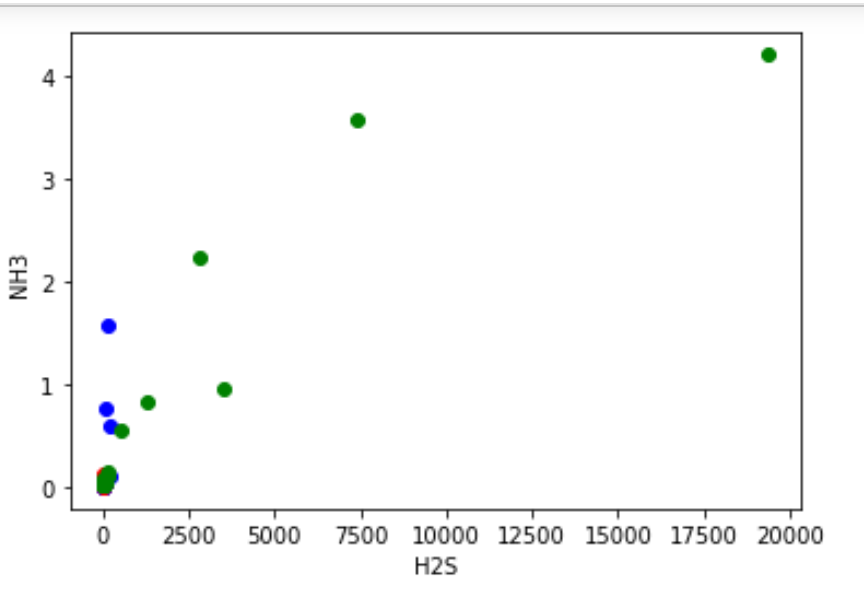
\includegraphics[width=0.5\textwidth]{pic/NH3_H2S.png}
		\end{figure}
		值得注意的是,許多紅點(3 \textasciitilde \ 6小時)的數據都在最左下角,被綠色覆蓋,直到七小時才會比較有明顯往外增加。
		我們推論是到較多小時後,雖然兩種氣體濃度都會明顯增加,但是差距也明顯,因此有時候即使濃度增加了,也還是很靠近圖中的原點。
